\section{Preliminaries}
\subsection{Citing MetaOmics}
MetaOmics software suite implements many meta-analytic methodologies by many different authors. 
Please cite appropriate papers if you used MeteOmics,
by which the authors will receive professional credits for their work.

\begin{itemize}
\item MetaOmics software suite  itself can be cited as: Ma et al. MetaOmics: Comprehensive Analysis Pipeline and Browser-based Software Suite for Transcriptomic Meta-Analysis.
\item MetaQC: \bibentry{kang2012metaqc}.
\item MetaDE: 
\begin{itemize}
\item \bibentry{fisher1925statistical}.
\item \bibentry{li2011adaptively}.
\item \bibentry{choi2003combining}.
\item and many more
\end{itemize}
\item MetaPath: 
\begin{itemize}
\item \bibentry{shen2010meta}.
\item \bibentry{fang2016cpi}.
\end{itemize}
\item MetaClust: \bibentry{huo2016meta}.
\item MetaPCA: \bibentry{kim2017metaPCA}.
\item MetaPredict: \bibentry{Kim2016}.
\item MetaNetwork: \bibentry{zhu2016metadcn}.
\end{itemize}



\subsection{How to start MetaOmics}

The full instruction of how to install, start MetaOmics software suite is also available at \url{https://github.com/metaOmics/metaOmics}.


\subsubsection{Requirement}
\begin{itemize}
\item R $>=$ 3.3.1
\item Shiny $>=$ 0.13.2
\end{itemize}

\subsubsection{How to install the metaOmics software}
\begin{itemize}
\item At MetaOmics home page at \url{https://github.com/metaOmics/metaOmics}, clone the project by
clicking on ``Clone or download" and extract to a working directory, 
or type in the following in command line

\textit{git clone} \url{https://github.com/metaOmic/metaOmics}
\end{itemize}

\subsubsection{How to start the metaOmics software}
\begin{itemize}
\item In R (suppose the application directory is metaOmics),

\textit{install.packages(`shiny')}

\textit{shiny::runApp(`metaOmics', port=9987, launch.browser=T)}
\end{itemize}

\subsection{MetaOmics setting page}
\label{sec:setting}
After starting MetaOmics, 
the first page is the MetaOmics setting page as shown in Figure~\ref{fig:GUIsetting}.  
There are 4 tabs on top of the page (at position {\color{red} (1)}): Setting, Preprocessing, Saved Data and Toolsets.
The welcome page is below the 4 tabs.
Further below, the first header is the session information.
{
\color{blue}
Why do we need session information?
}
The second header is Directory for Saving Output Files (at position {\color{red} (2)}).
By clicking ``$\ldots$",
user can set default working directory, in which all the meta-analysis results will be saved.
Users can view their current working directory on the top right corner (at position {\color{red} (3)}).
The third header is Toolsets (at position {\color{red} (4)}),
where user can click to install desired modules if the ``status" shows ``not installed".
If the packages are installed, there is a checked installed status.
Otherwise, users can install individual package by clicking install blue button.
The installation progress may take a few minutes for each module.
There will be a notification icon at the bottom right corner after the installation. 
After the modules are installed to R, restart the MetaOmics software suit so that the shiny application interface is updated with installed modules.
Position {\color{red} (5)} shows the current active dataset, which will be introduced in Section~\ref{sec:procedure}~\ref{sec:active}. 
 
\begin{figure}[H]
\begin{center}
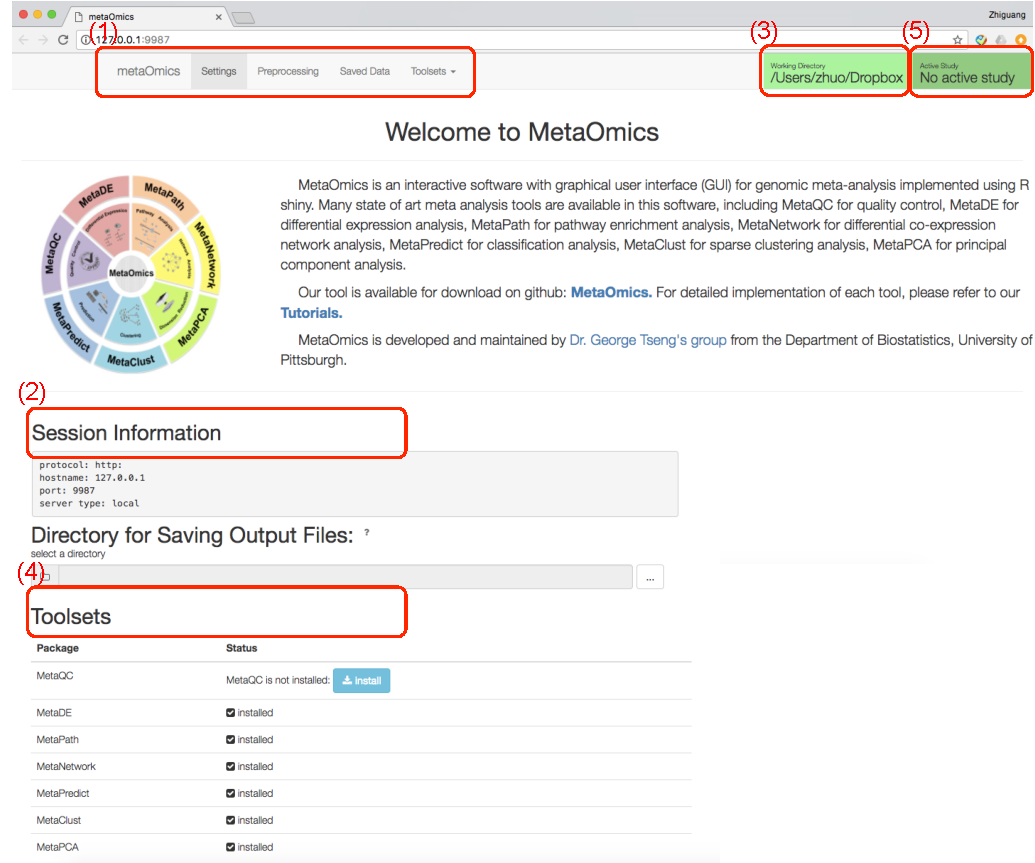
\includegraphics[scale=0.8]{./figure/preprocessing/GUIsetting}
\caption{MetaOmics software suite GUI setting page}
\label{fig:GUIsetting}
\end{center}
\end{figure}


\subsection{Question and bug report}
{
\color{red}
Who should be responsible for maintaining the software?
}

 
